\section{Machine Learning}
\subsection{Introduction}
Machine learning, also known as statistical learning is the study of different types of algorithms. 
\begin{quote}
\textit{It's an integral part of many commercial applications and research projects today, in area ranging from medical diagnosis and treatment to finding your friends on social network.} \cite{muller_guido_2016}
\end{quote}
Several stages are involved in the machine learning process where it starts with identifying the problem followed by data collection, data analysis and pre-processing, feature extraction, machine learning model development and ends with performance evaluation of the model. The model would then be deployed after achieving a rather good performing benchmark.
Machine learning can be divided further into three classes which are unsupervised learning, supervised learning and reinforcement learning. In a supervised learning algorithm, each data set provided belongs to a particular class. In simple terms, an input variable, x exists along with an output variable, y where the algorithm will map the input variable to the output variable. This concept can be expressed with a simple equation in \ref{eq:1}. 
\begin{equation}
    y = f(x)  \label{eq:1}
\end{equation}
Moreover, supervised learning can be further broken down into classification and regression. Classification is used to classify or predict the class of each data while regression is used to predict a continuous output variable from a number of independent variables \cite{abrams_2007}. Examples of supervised learning algorithms are k-nearest neighbour (kNN), support vector machine (SVM) and XGBoost.  

Next, unsupervised learning algorithms are used to study pattern of datasets which do not have labels or classes. Clustering and anomaly detection are examples of unsupervised learning. “On the other hand, reinforcement learning is a process of training machine learning models giving them the ability to make decisions in a sequence” \cite{osinski_budek_2018}. 

\subsection{Processes}
\subsubsection{Data Collection, Analysis and Pre-processing}
Before training and building a machine learning model, a problem should be identified and defined. Datasets related to the problem are then collected, analysed and pre-processed. Data collected can exist in the form of categories, time-series, text and numbers. Datasets collected contain a large number of features most of the time and useful features are only required. Therefore, data analysis is carried out to search for correlation between features and the target variables or classes. Several data analysis methods can be carried out such as producing a correlation matrix, histograms, bar plots and scatter plots \cite{kashnitsky_2019}.

A correlation matrix shows the coefficient between two parameters in a N x N matrix where N represents the number of parameters. The Pearson's correlation coefficient is used and represented with the symbol \textit{r} and exist in the range of $-1\leq r \leq 1$. It measures the strength and linear relationship between two variables \cite{corr}.  The strengths of the correlation coefficients can be shown in table \ref{table:corr}. 

\begin{table}[h!]
\centering
\begin{center}
\begin{tabular}{ |c|c| } 
 \hline
 Correlation coefficient & Correlation strength\\ 
  \hline\hline
 1.0 & Very strong positive relationship\\ 
 0.8 & Fairly strong positive relationship\\ 
 0.6 & Moderate positive relationship\\ 
 0 & No relationship\\ 
 -0.6 & Moderate negative relationship\\ 
 -0.8 & Fairly strong negative relationship\\ 
 -1.0 & Very strong negative relationship \\ 
  
 \hline
\end{tabular}
\caption{Correlation coefficients strength}
\label{table:corr}
\end{center}
\end{table}
In the data pre-processing stage, anomalies would be removed. For missing data values, they are either removed or replaced with a null value. Time-series data that exists as signals will be filtered to remove unwanted noise or frequencies. The data would then be normalized or standardized to obtain data uniformity. Normalization is a process that scales values to a range between 0 and 1 while standardization scales values to be centered around the mean with a standard deviation of 1 \cite{norm_stand}. These processes are usually effective on distance-based algorithms such as k-NN. 

\subsubsection{Training, Validating and Testing phases}
The training, validation and testing phases will be performed with the preprocessed and filtered data with useful features. The dataset prepared is commonly split into ratios of 90:10 where 90\% of the data will be further split into a 80:10 ratio that will be used to train and validate the machine learning model and 10\% of the remaining data will be used to test and evaluate the built model. Other commonly used ratios used include 70:15:15 and 60:20:20. A validating set is used to evaluate the model which allows users to tune the hyperparameters to achieve a better performance. The final performance of the trained model will then be evaluated with the test data. 
\subsection{Supervised Algorithms}

\subsubsection{k-Nearest Neighbour}
K-nearest neighbour is a simple supervised learning algorithm that is frequently used for classification and regression problems. This algorithm works by simply storing the training dataset provided. It predicts or classifies a new data point by searching for the closest data points in the training data set - its ``nearest neighbors'' \cite{muller_guido_2016}.

The hyperparameters that are used for this algorithm are the distance function and number of neighbours, k. The number of neighbours is a parameter which takes the \textit{k} closest training points in the model to predict or classify a given test point. A distance function is the measure of distance to map a training point to a test point. Several examples of distance functions used are the Manhattan, Euclidean and Minkowski distance functions. The Euclidean distance function is widely used and is said to represent the shortest distance between two points in a N-dimensional space. The corresponding function can be represented by the expression in 
\ref{eq:2} \cite{knn} where x represents the training point of the model, y represents a test point while n represents the dimension of the vector space (no. of features). 
\begin{equation}
    d(x,y) = \sqrt{(x_1^2-y_1^2)+(x_2^2-y_2^2)+....+(x_n^2-y_n^2)} \label{eq:2}
\end{equation}

An example where two classes, class A and class B exist in a trained k-NN model is shown in \ref{fig_knn}. The model with a \textit{k} value of 1 classifies a new data point by mapping the closest one training point from Class A to the test point.

\begin{figure} [ht]
    \centering
    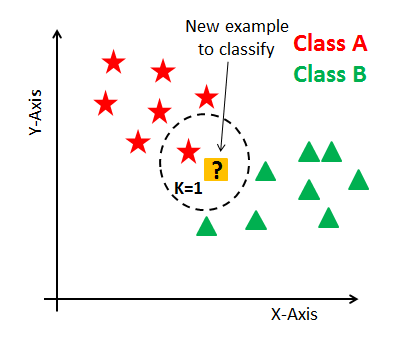
\includegraphics[scale=0.6]{pages/Chapter2/Chapter 2 images/knn.png}
    \caption{Classification of a test point with kNN. \textit{Sourced from} \cite{chauhan_2019}.}
    \label{fig_knn}
\end{figure}
 
\subsubsection{XGBoost}
XGBoost which is also known as ``\textit{e\textbf{X}treme \textbf{G}radient \textbf{B}oosting}" is a type of supervised learning algorithm used in machine learning. It is the implementation of gradient boosting machines or boosted decision trees where it heavily focuses on optimization and scalability. The XGBoost algorithm is used to solve regression and classification problems. This algorithm uses the concept of decision trees where features are split further into intervals to classify data in the form of nodes and branches.

The hyperparameters of this algorithm includes the number of classes involved, learning rate, gamma and subsamples. The number of classes represents the number of target variables available in the data provided. The learning rate prevents the overfitting of data where the trained model is only able to predict values that exist in the the training set.
Overfitting implies that the model trains by including noise or existing anomalies in the provided dataset. The subsample and gamma hyperparameter shares the similar concept as well to prevent overfitting of the machine learning model. 

\subsection{Machine Learning Model Performance Evaluation}
The final performance of the machine learning model will be evaluated using the split test data. Metrics such as the confusion matrix can be used to measure the performance of the trained model. Several parameters can be obtained from the confusion matrix such as accuracy, sensitivity, precision and specificity. The confusion matrix is a N x N matrix which shows the number of classified and misclassified data for N classes of data. An example of a confusion matrix can be shown in \ref{fig_cf}.

\begin{figure} [ht]
    \centering
    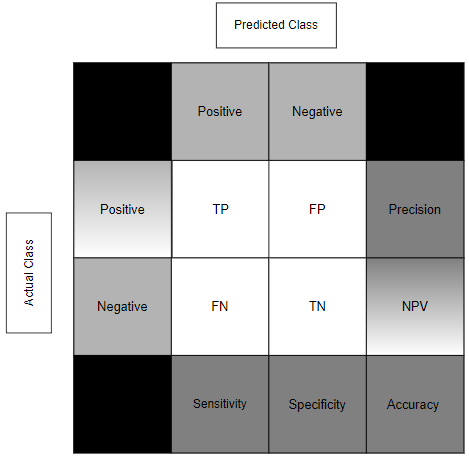
\includegraphics[scale=1.0]{pages/Chapter2/Chapter 2 images/Confusion matrix.PNG}
    \caption{Confusion matrix.}
    \label{fig_cf}
\end{figure}

From fig. \ref{fig_cf}, TP, FP, FN and TN represents true positive, false positive, false negative and true negative respectively. True positive and true negative represent data predicted correctly with the actual class while false positive and false negative are misclassified data predicted under the incorrect class.
The accuracy of the model which represents the data are classified under the correct class can be evaluated with \ref{eq:3}.
\begin{equation}
    Accuracy(\%) = \frac{TP + TN}{TP+TN+FN+FP} \times 100\% 
    \label{eq:3}
\end{equation}

Precision measures the frequency of data predicted correctly under the positive class as shown in \ref{eq:4} \cite{metrics}. For instance, a precision value of 0.7 defines that when the classifier predicts a data point under the true positive class, it has a 70\% chance of classifying it correctly.
\begin{equation}
    Precision(\%) = \frac{TP}{TP+FP} \times100\% 
    \label{eq:4}
\end{equation}

Sensitivity shows the proportion of data classified correctly under the positive class and can be computed  with \ref{eq:5} \cite{metrics}. It is also known as recall. For example, a recall value of 0.9 would mean that the classifier correctly predicts 90\% of the true positive class. 
\begin{equation}
    Sensitivity(\%) = \frac{TP}{TP+FN} \times100\% 
    \label{eq:5}
\end{equation}

F1-score is a function of precision and recall where it is a metric which provides balance between those two parameters. Since a good performing model would have high precision and recall, this metric summarizes them together into a single value. The F1-score is calculated as shown in \ref{eq:6} \cite{metrics}.
\begin{equation}
   F1-score = \frac{2\times Precision\times Recall}{Precision+Recall} \times100\% 
    \label{eq:6}
\end{equation} 

Thus, the confusion matrix is one of the several useful metrics to determine the performance of a machine learning model before getting it ready for deployment.



